%!TEX TS-program = xelatex
\documentclass[]{friggeri-cv}
\usepackage{afterpage}
\usepackage{hyperref}
\usepackage{color}
\usepackage{xcolor}
\usepackage{smartdiagram}
\usepackage{fontspec}
% if you want to add fontawesome package
% you need to compile the tex file with LuaLaTeX
% References:
%   http://texdoc.net/texmf-dist/doc/latex/fontawesome/fontawesome.pdf
%   https://www.ctan.org/tex-archive/fonts/fontawesome?lang=en
%\usepackage{fontawesome}
\usepackage{metalogo}
\usepackage{dtklogos}
\usepackage[utf8]{inputenc}
\usepackage{tikz}
\usetikzlibrary{mindmap,shadows}
\hypersetup{
    pdftitle={},
    pdfauthor={},
    pdfsubject={},
    pdfkeywords={},
    colorlinks=false,           % no lik border color
    allbordercolors=white       % white border color for all
}
\smartdiagramset{
    bubble center node font = \footnotesize,
    bubble node font = \footnotesize,
    % specifies the minimum size of the bubble center node
    bubble center node size = 0.5cm,
    %  specifies the minimum size of the bubbles
    bubble node size = 0.5cm,
    % specifies which is the distance among the bubble center node and the other bubbles
    distance center/other bubbles = 0.3cm,
    % sets the distance from the text to the border of the bubble center node
    distance text center bubble = 0.5cm,
    % set center bubble color
    bubble center node color = pblue,
    % define the list of colors usable in the diagram
    set color list = {lightgray, materialcyan, orange, green, materialorange, materialteal, materialamber, materialindigo, materialgreen, materiallime},
    % sets the opacity at which the bubbles are shown
    bubble fill opacity = 0.6,
    % sets the opacity at which the bubble text is shown
    bubble text opacity = 0.5,
}

\addbibresource{bibliography.bib}
\RequirePackage{xcolor}
\definecolor{pblue}{HTML}{0395DE}

\begin{document}
\header{Rubén}{Tobar Nicolau}
      {Graduado en Ingeniería Informática}
      
% Fake text to add separator      
\fcolorbox{white}{gray}{\parbox{\dimexpr\textwidth-2\fboxsep-2\fboxrule}{%
.....
}}

% In the aside, each new line forces a line break
\begin{aside}
  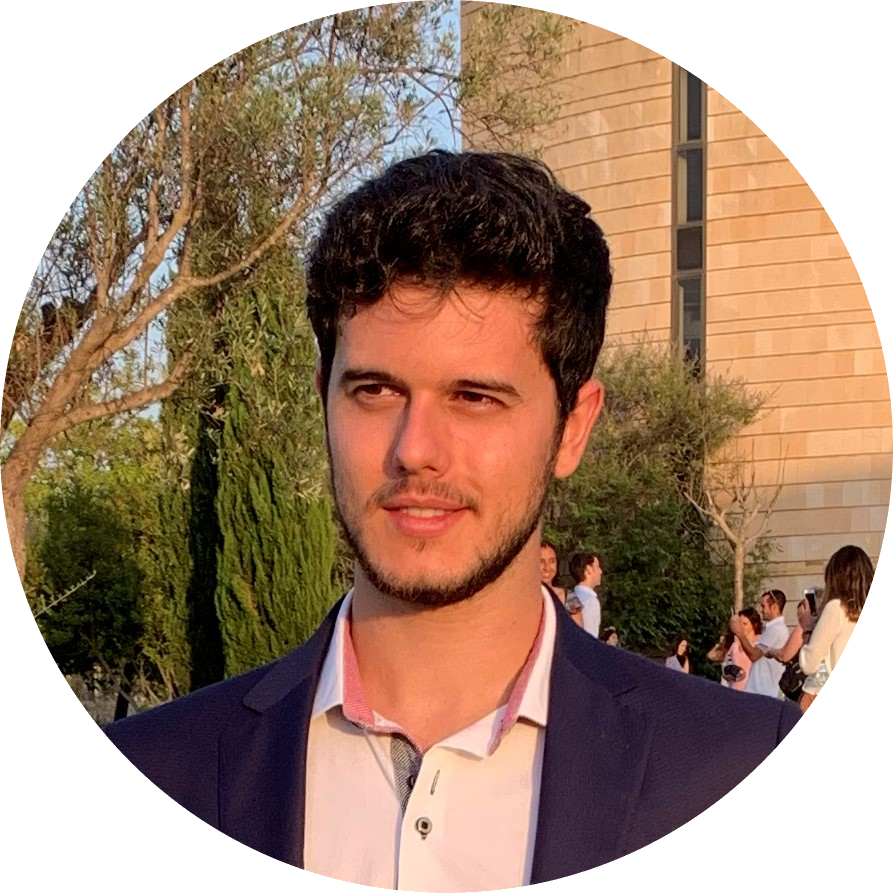
\includegraphics[scale=0.17]{img/yo.png}
  \section{Datos personales}
    DNI: 43223519X
%    Fecha nacimiento: 09-10-1995
    ~
  \section{Dirección}
    Madrid
    ~
  \section{Tel \& Skype}
    +34 677 119139
    Skype: mc-tobar
    ~
  \section{Mail \& Linkedin}
    \href{mailto:rntobar41@gmail.com}{\textbf{rntobar41@}\\gmail.com}
    \href{https://www.linkedin.com/in/rubén-tobar-nicolau-84761117a}{\textbf{linkedin.com/in/rubén-tobar-nicolau-84761117a}}
    ~
  \section{Git - proyectos personales}
    %\href{http://mywebsite.com}{mywebsite.com}
    \href{https://github.com/rubtobar}{github.com/rubtobar}
    \href{https://gitlab.com/rubtobar}{gitlab.com/rubtobar}
    ~
  % use  \hspace{} or \vspace{} to change bubble size, if needed
  \section{Tecnologías}
        Java, C\#, C, C++
        Python
        HTML, CSS, JS, PHP
        Kubernetes, Docker
        nodejs, Angular, TensorFlow
    ~
    \section{Idiomas}
     \textbf{Español (Nativo)}
     \textbf{Inglés (Alto)}
     \textbf{Catalán (Nativo)}
    ~
\end{aside}
~
\section{Experiencia Laboral}
\begin{entrylist}
  \entry
    {08/17 - 10/17}
    {Ingeniero Informático}
    {Juniper Innovating Travel Technology}
    {Prácticas como Project Manager en empresa con alcance mundial. Empresa enfocada en el sector turístico. Juniper provee de una booking engine, desarrollada por la empresa, para la venta de producto turístico tanto B2B como B2C.}
\end{entrylist}

\begin{entrylist}
  \entry
    {03/20 - Act. }
    {Ciberseguridad ISDEFE}
    {Beca en Ingeniería de Sistemas para la Defensa de España}
    {ISDEFE, es una empresa pública de consultoría e ingeniería, medio propio y servicio técnico, de referencia en el ámbito de Defensa y Seguridad, de la Administración General del Estado. ISDEFE ofrece servicios a organismos públicos nacionales e internacionales en áreas de interés tecnológico y estratégico.}
\end{entrylist}

\section{Formación}
\begin{entrylist}
  \entry
    {2013 - 2019}
    {Grado en Ingeniería Informática}
    {Universidad de las Islas Baleares}
    {
    Mención en computación. \\
    Este grado está acreditado con el sello EURO-INF, la acreditación internacional de ingeniería informática más prestigiosa de Europa, otorgada por la Red Europea de Garantía de la Calidad de la Educación en Informática (EQANIE). Esta acreditación garantiza que la titulación cumple los elevados estándares de calidad fijados por la EQANIE.}
\end{entrylist}

\begin{entrylist}
  \entry
    {2020 - 2021}
    {Titulación CITIUS by FUE}
    {Universidades Autónoma de Madrid y de Barcelona}
    {
    La beca se ha realizado en el Mando Conjunto de Ciber Defensa en la empresa ISDEFE conjuntamente con cursos de la Universidades Autónoma de Madrid, correspondientes a 18CTS. }
\end{entrylist}


%\section{Publications}
%Author, Author, Author\\
%\textbf{Lorem ipsum dolor sit amet, consectetur adipiscing elit, sed do eiusmod tempor incididunt %ut labore et dolore magna aliqua}\\
%\emph{Lorem ipsum dolor sit amet, consectetur adipiscing elit, sed do eiusmod tempor incididunt %ut labore et dolore magna aliqua}
%\\
\section{Proyectos}
\begin{entrylist}
  \entry
    {07/2019}
    {Proyecto de final de carrera}
    {Universidad de las Islas Baleares}
    {Estudio sobre inteligencia artificial y redes neuronales generativas antagónicas (GAN). Estudio del funcionamiento de las redes GAN y diseño de un generador capaz de sintetizar figuras del silabario japonés del siglo 18. Estudio sobre la capacidad de aprendizaje de la red al aumentar la complejidad de los datos. \\
    \emph{Evaluado por tribunal con calificación de 9.5/10.0}}
\end{entrylist}

\section{Estancias en el extranjero}
\begin{entrylist}
  \entry
    {2011}
    {Winchester, Reino Unido}
    {Education First exchange}
    {\emph{Estancia de un mes con clases de inglés diarias.}}
  \entry
    {2017}
    {Bologna, Italia}
    {ERASMUS+}
    {\emph{Estancia de 6 meses en Italia en la universidad Alma Mater Stodiorum Università di Bologna.}}
\end{entrylist}

%\begin{flushright}
%\emph{Rubén Tobar Nicolau}
%\end{flushright}


%\begin{aside}

%  \section{OS Preference}
%    \textbf{GNU/Linux}
\includegraphics[scale=0.40]{img/5stars.png}
%    \textbf{Unix}
\includegraphics[scale=0.40]{img/4stars.png}
%    \textbf{MacOS}
\includegraphics[scale=0.40]{img/2stars.png}
%    \textbf{Windows}
\includegraphics[scale=0.40]{img/1stars.png}
%    ~
%  \section{Places Lived}
%    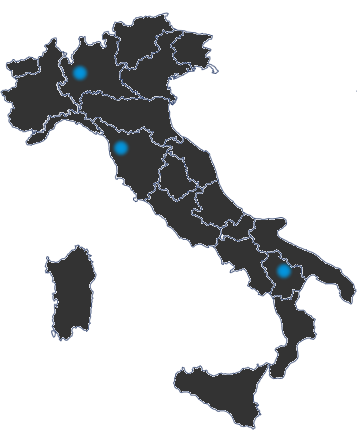
\includegraphics[scale=0.25]{img/italia.png}
%    ~

%\end{aside}



\end{document}
